\documentclass[11pt]{report}

% report format
\usepackage[hidelinks]{hyperref}
\usepackage[utf8]{inputenc}
\usepackage[a4paper, top=3cm, bottom=3cm, left=3.5cm, right=3cm]{geometry}
\usepackage{setspace}
\onehalfspacing{}
\usepackage{chngcntr}
\counterwithout{footnote}{chapter}
\usepackage{fancyhdr}
\fancyhead[L]{\leftmark}
\fancyhead[C,R]{}
\usepackage{graphicx}
\usepackage{tabu}
\tabulinesep=_4pt

% reference
\usepackage[style=ieee]{biblatex}
\addbibresource{../sources.bib}

% code listings
\usepackage{listings}
\usepackage{color}
\definecolor{codegreen}{rgb}{0,0.6,0}
\definecolor{codegray}{rgb}{0.5,0.5,0.5}
\definecolor{codepurple}{rgb}{0.58,0,0.82}
\definecolor{backcolour}{rgb}{0.95,0.95,0.92}
\lstdefinestyle{mystyle}{
    backgroundcolor=\color{backcolour},
    commentstyle=\color{codegreen},
    keywordstyle=\color{magenta},
    numberstyle=\tiny\color{codegray},
    stringstyle=\color{codepurple},
    basicstyle=\footnotesize\ttfamily,
    breakatwhitespace=false,
    breaklines=true,
    captionpos=b,
    keepspaces=true,
    % numbers=left,
    numbersep=5pt,
    showspaces=false,
    showstringspaces=false,
    showtabs=false,
}
\lstset{style=mystyle}

% actual report
\pagenumbering{gobble}
\begin{document}
\begin{titlepage}
\begin{center}

% school logo

\includegraphics[width=0.9\textwidth]{images/ntu_logo.png}
\\[5cm]

% report title
\uppercase{\textbf{Final Year Project Interim Report}}
\\[5cm]

% submited by ...
\uppercase{\textbf{Nguyen Huy Anh}}

\vfill

% Bottom of the page
\textsc{\bfseries School of Computer Science and Engineering}
\\
\textbf{Academic Year 2017/18}

\end{center}
\end{titlepage}

\begin{titlepage}
\begin{center}

\uppercase{\textbf{Nanyang Technological University}}
\\[5cm]

\uppercase{
    \textbf{SCE16--0550}\\
    \textbf{A Multimedia Transcription System}
}\\[5cm]

Submitted in Partial Fulfillment of the Requirements\\
for the Degree of Bachelor of Engineering (Computer Science)\\
of the Nanyang Technological University\\[1cm]
by\\[1cm]
Nguyen Huy Anh\\
(U1420871B)

\vfill

\textbf{School of Computer Science and Engineering}\\
\textbf{Academic Year 2017/18}

\end{center}
\end{titlepage}

\pagenumbering{roman}
% Front matter
\phantomsection{}
\addcontentsline{toc}{chapter}{Abstract}
\chapter*{Abstract}
With the advent of computing, a huge amount of data is being created everyday.
Most of the data are unstructured or semi-structured, and needs to be processed
in order to derive meaning. For multimedia data (audio and video), a textual
representation is often desirable, and there are two ways to obtain such a
representation --- transcription and captioning. The two processes are
well-defined pipelines of multiple components.

However, for each component there are many existing implementations, but each
having differentiated input and output formats, which makes it difficult to
integrate to a pipeline. The pipeline itself is difficult to maintain, with
any change/ upgrade to any component having a potential to break the pipeline.
Furthermore, as the pipeline changes there is no mechanism to keep track of
output versions; this capability is important for research purposes.

This project proposes an integrated processing system performing transcription
and captioning on a wide range of audio and video inputs --- single-file audio/
video as well as multi-channel audio recordings. The project aims to design
a system architecture that allows for modularity and extensibility, keeps track
of different component and output versions and performs robustly under many
scenarios. The project incorporates Python ports of existing modules from various
efforts of the Speech and Language Research Group in the School of Computer
Science and Engineering, as well as new Python modules to realize the processing
pipeline --- transcription, captioning and visualizations of transcripts and
captions.

The project would be evaluated on existing audio records of talk shows 
(Singapore's 93.8FM), video records (Singapore Parliament proceedings) and
multi-channel recordings (a four-people conversation on Singapore Army). It
achieves all the requirements and proves the usefulness of this project.

\newpage

\phantomsection{}
\addcontentsline{toc}{chapter}{Acknowledgements}
\chapter*{Acknowledgements}
This Final-Year Project would not have been successful without the support
of my mentors, reviewers, friends and family.

Above all, I would like to extend my most sincere gratitude to my supervisor,
Associate Professor Chng Eng Siong for your guidance throughout
the course of this project and beyond.

I would also like to thank the research staff of the Speech
and Language Research Group at the School of Computer Science and Engineering,
Nanyang Technological University for your support in many of the project's
deliverables. The specific persons, in no particular order, are, Dr.\ Xu Haihua,
Mr.\ Kyaw Zin Tun, Mr.\ Pham Van Tung, Ms.\ Ho Thi Nga, and Ms.\ Vu Thi Ly.

Finally, I would like to say thanks to my friends and family, especially to my
dearly beloved, for your emotional support during this period and throughout my
university education.
\newpage

\phantomsection{}
\addcontentsline{toc}{chapter}{Table of Contents}
\tableofcontents
\newpage

\phantomsection{}
\addcontentsline{toc}{chapter}{List of Figures}
\listoffigures
\newpage

\phantomsection{}
\addcontentsline{toc}{chapter}{List of Tables}
\listoftables
\newpage

\phantomsection{}
\addcontentsline{toc}{chapter}{List of Abbreviations}
\chapter*{List of Abbreviations}
\begin{tabu}{lX}
    \textbf{API} & Application Programming Interface \\
    \textbf{CLI} & Command-line Interface \\
    \textbf{GUI} & Graphical User Interface \\
    \textbf{LVCSR} & Large Vocabulary Continuous Speech Recognition \\
    \textbf{PCM} & Pulse-code Modulation \\
    \textbf{SLRG} & Speech and Language Research Group at School of Computer
    Science and Engineering \\
    \textbf{VAD} & Voice Activity Detection
\end{tabu}
\newpage

\pagenumbering{arabic}
\pagestyle{fancy}
\chapter{Introduction}

\section{Background}

With the advent of computing, a large amount of data is being created everyday.
Raw data exists in many forms --- numbers, texts, images, audio, video, etc.,
and it must be processed in order to derive meaning. For multimedia data (audio
and video), a textual representation of the data is desirable as a pre-cursor
to further processing. The process of converting speech to text is called
transcription; the resultant transcript could be utilised in other tasks ---
archival, indexing and search, concept and language understanding, etc.

Transcription is a well-defined pipeline:

\begin{figure}[h]
\begin{center}
    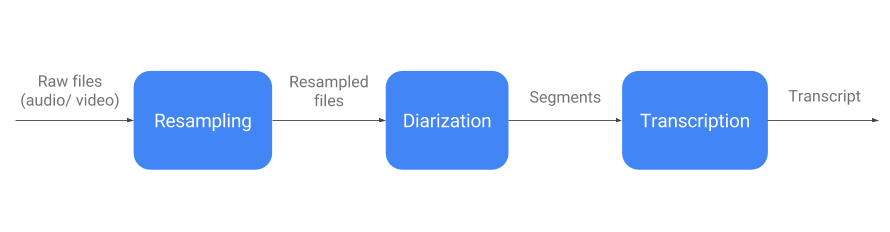
\includegraphics[width=0.9\textwidth]{../images/pipeline.png}
    \caption{Transcription processing pipeline}
\end{center}
\end{figure}

Transcription starts with the raw audio or video file, which could be
single-speaker (for example lecture recordings, Parliament speeches) or
multi-speaker (for example conversations, talk shows). The file is then resampled
to an appropriate configuration of bit rate and sample size. The resampled audio
goes through the process of speaker diarization, to separate different audio
segments (usually short) said by different speakers. These short segments are
then fed one-by-one to a transcription system; combining all the results gives
the final transcript.

For each process in the pipeline, there exists multiple solutions to perform
the task. Many of them are either public APIs or open-source; however, they exist
as ``black boxes'' --- each solution accepts input and produces output in a
specific manner. This presents a challenge in integrating multiple solutions to
realise the transcription pipeline. Additionally, given an integrated pipeline,
upgrading or changing any component could potentially break the pipeline. After
the pipeline is upgraded, there must also be a mechanism to update the
transcriptions and keep track of versions. 

This project proposes an integrated transcription system; apart from realising
the transcription pipeline, this system would be able to accommodate versioning
of all the pipeline components as well as all the transcripts. Ultimately, this
results in a simple and more efficient processing workflow for multimedia.

This project would be done in conjunction with other efforts of the Speech and
Language Technology Group in School of Computer Science and Engineering
(thereafter referred to as SLTG).

\section{Objective}

The primary objective of this project is to design a system architecture and
develop the respective system capable of performing the following tasks:

\begin{itemize}
    \item Transcription of individual audio and video files using different
    transcription solutions
    \item Transcription of multi-channel audio recording
\end{itemize}

The developed system must also have the following qualitative requirements:

\begin{itemize}
    \item Modularity --- allowing independent component operation and low coupling
    \item Extensibility --- allowing system extension to perform other related
    tasks in audio and video processing
    \item Robustness --- allowing system error recovery and process resumption
    \item Versioning --- allowing for different results with different processing
    components, and enabling evaluation of different components
    \item Logging and Reporting --- allowing developers to understand and generate
    insights to the outputs
\end{itemize}

\section{Scope}

The scope of this project is restricted to developing a system to be used in a
desktop/ laptop Ubuntu Linux environment, to perform the tasks mentioned above. A
functioning graphics user interface (GUI) is also not required.

However, the system could be modified and extended to perform other related tasks
in different environments, with a GUI\@.

\section{Project Timeline}

The project was scheduled to commence from January 2017 to October 2017. The major
milestones are as follows:

\begin{itemize}
    \item \textbf{End of January 2017:} Completion of Architectural Design
    \item \textbf{End of April 2017:} Completion of Porting of Existing Modules
    to Current System
    \item \textbf{End of September 2017:} Completion of Development of New Modules;
    Commencement of Integration Testing
    \item \textbf{End of October 2017:} Completion of Project
\end{itemize}

\section{Report Organisation}

This report is divided into four chapters:

\begin{itemize}
    \item Chapter 1 provides an introduction to the project, states its objective
    and scope and provides a timeline for completion.
    \item Chapter 2 gives a summary of the work done so far on the project
    \item Chapter 3 gives an overview to the remaining work to be done before the
    project completes.
    \item Chapter 4 concludes the report.
\end{itemize}
\printbibliography{}
\end{document}
